\section{Verification and numerical resolution}
\label{sec:verification}

We compare the implementation with analytical limits, independent transfer-matrix calculations, algebraic identities, and mesh-refinement results. For the published heterogeneous bilayers, we report only qualitative graphical agreement where source curves are available. Cases with ambiguous parameters or no numerical curves are not treated as external validation.

\subsection{Analytical limits and bilayer comparison}
In the isotropic homogeneous limit, the long-wavelength phase velocities recover the classical transverse and longitudinal speeds:
\begin{equation}
\lim_{k\to0}\frac{\omega_T(k)}{k}=\sqrt{\frac{\mu}{\rho}}=1.0,\qquad
\lim_{k\to0}\frac{\omega_L(k)}{k}=\sqrt{\frac{\lambda+2\mu}{\rho}}=\sqrt{3}\approx1.73205.
\label{eq:acoustic_limits}
\end{equation}
At $\bar{k}=0.001$, the computed acoustic speeds differ from these limits by $1.25\times10^{-8}$ (Table~\ref{tab:consistency_suite}). The pure-bending micro-beam reduction matches the published closed-form limits to within $10^{-15}$ \cite{papargyribeskou2009}; details appear in Supplementary Material~S2. The micro-inertia asymptote is checked separately in \ref{app:asymptotics} and Section~\ref{sec:microinertia}.

As a classical reference, we analyze a periodic AlN/BaTiO$_3$ bilayer with $a_A=a_B=0.01\,\mathrm{m}$ and $b=a_A+a_B=0.02\,\mathrm{m}$ using the Rytov relation \cite{li2024anchorB,zhengwei2009}:
\begin{equation}
\cos(Kb)=\cos(k_Aa_A)\cos(k_Ba_B)-\frac{1}{2}\left(\frac{Z_A}{Z_B}+\frac{Z_B}{Z_A}\right)\sin(k_Aa_A)\sin(k_Ba_B),
\label{eq:rytov}
\end{equation}
where $k_m=\omega\sqrt{\rho_m/c_{33,m}}$, $v_m=\sqrt{c_{33,m}/\rho_m}$, and $Z_m=\rho_m v_m$. The single-layer transfer-matrix identity and the identical-material bilayer reduction match their analytical limits to $6.47\times10^{-16}$ and $7.22\times10^{-16}$, respectively. The heterogeneous transfer-matrix trace reproduces the Rytov relation to $2.22\times10^{-16}$. The first three calculated stop-band intervals are $[0.4806,0.5209]$, $[0.9812,1.0215]$, and $[1.4993,1.5028]$ in normalized frequency. We compare the result with the published B1 plot visually because tabulated source data are unavailable; no percentage error is inferred from the curves.

We reproduce two gradient-elastic bilayer cases, but do not treat them as external validations. One published length-scale definition is dimensionally ambiguous. For the other, the plotted parameter set and normalization are unspecified, and the numerical curves are unavailable. Supplementary Material~S2 records these limitations and the status of each comparison. We also compare the dipolar layer matrix with the source's printed formulation; this checks the formulation but does not validate its band curves.

\subsection{Numerical consistency and mesh convergence}
The consistency checks assess operator Hermiticity, Brillouin-zone periodicity, isotropic rotational invariance, acoustic slopes, rotation--swap symmetry, matrix definiteness, the micro-inertia limit, and the energy-flux/group-velocity identity. Table~\ref{tab:consistency_suite} reports the values obtained for these comparisons. After the harmonic micro-inertia sign correction in Appendix~\ref{app:energy_flux}, the energy-flux residual cannot be independently recalculated because the raw harmonic fields are unavailable. We therefore retain this identity as an unresolved diagnostic rather than treating the reported residual as independent confirmation. Supplementary Material~S3 gives the check definitions and expanded diagnostics.

We assess mesh convergence for homogeneous Case~H on uniform $N\times N$ BFS grids, $N\in\{4,8,16,32\}$, at fixed $\bmk=(0.31\pi/L,0.22\pi/L)$. Figure~\ref{fig:mesh_convergence} shows the acoustic-frequency error relative to the closed-form value and the change between successive meshes. The fitted empirical rate is $p=4.17$ (95\% CI $[3.15,5.20]$) over the $4^2$, $8^2$, and $16^2$ levels. The reported $32^2$ result is resolution-limited and is excluded from the fit. This rate is empirical; it is not a theoretical-order claim. The operational mesh-change floor is $\varepsilon_\Delta=4.63\times10^{-11}$ and is distinct from eigensolver reproducibility. The smallest reported directional gap, $|\Delta_{GX}|=4.3\times10^{-3}$, exceeds the floor by approximately $9\times10^7$.

\begin{figure*}[!t]
\centering
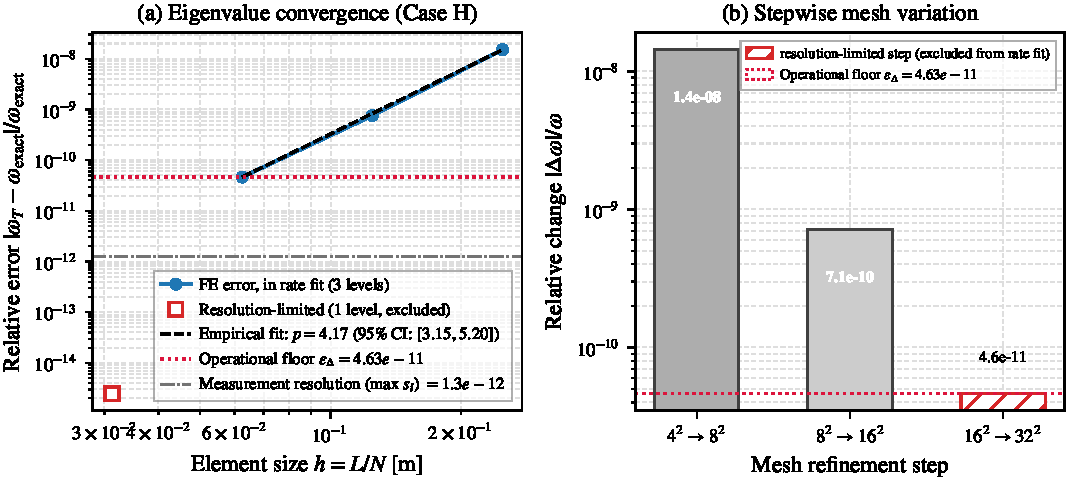
\includegraphics[width=\textwidth]{figures/fig05_mesh_convergence.pdf}
\caption{Case-H mesh study for the acoustic branch. (a) Relative frequency error versus element size; the $32^2$ result is shown as resolution-limited and is not included in the empirical fit. (b) Successive-mesh change and the operational mesh-change floor $\varepsilon_\Delta$.}
\label{fig:mesh_convergence}
\end{figure*}

\begin{table*}[!t]
\centering
\caption{Numerical consistency checks for the Bloch finite-element implementation.}
\label{tab:consistency_suite}
\begin{tabularx}{\textwidth}{@{}l Y c c c@{}}
\toprule
Check & Quantity assessed & Maximum discrepancy & Criterion & Result \\
\midrule
Hermiticity & Reduced stiffness and mass operators & $2.01\times10^{-16}$; $5.63\times10^{-17}$ & $<10^{-12}$ & Within criterion \\
Brillouin-zone periodicity & Spectrum under reciprocal-lattice shifts & $9.66\times10^{-16}$ & $<10^{-10}$ & Within criterion \\
Isotropic rotation & Frequencies at $\mathrm{AR}=1$ & $9.63\times10^{-16}$ & $<10^{-10}$ & Within criterion \\
Acoustic limit & Long-wave transverse and longitudinal slopes & $1.25\times10^{-8}$ & $<10^{-6}$ & Within criterion \\
Rotation--swap symmetry & Spectrum under $\theta\mapsto\theta+90^\circ$ and axis swap & $6.44\times10^{-16}$ & $<10^{-10}$ & Within criterion \\
Definiteness & Two rigid modes at $\Gamma$; positive interior spectrum & As expected & Admissible & As expected \\
Micro-inertia limit & Phase speed at $\bar{k}=200$ versus asymptotic value & $2.85\times10^{-4}$ & $<10^{-3}$ & Within criterion \\
Energy-flux identity & Group velocity versus cycle-averaged flux & $6.91\times10^{-10}$ & $<10^{-6}$ & Unresolved \\
\bottomrule
\end{tabularx}

\end{table*}

Selected Case-H and Case-C inputs appear with the Results. Supplementary Material~S1--S4 contains the full parameter summary, external-comparison details, and extended convergence diagnostics.
